\chapter{State Of The Art} 
\label{cha:sota}
This work combines the broad research field of thermal modeling of electric machines with the latest insights of machine learning and time series modeling via \glspl{ann}.
One can find a vast amount of contributions in both scientific areas in the literature, which lay the foundation of this thesis' investigation.
The considered research articles' publication years range from the early 80's to very recent time.
Most of the newer work requires solid knowledge of statistical modeling basics and model selection methodology.
Moreover, this work's field of application has well established formulae describing electric machine behavior on top of which research is conducted.

In order to ease reading of the matter and improve comprehensibility a brief background of the necessary fundamentals is given in the next sections.  
%First of all, a brief introduction to the \gls{pmsm} and its describing mathematical equations are given in section \ref{sec:pmsm}, which represents the basis on which benchmark data was measured.
%After that, the very basics of \glspl{ann} are explained and illustrated in section \ref{sec:ml_ann} with emphasis on the varying architectures, supervised learning algorithms and common model selection methods.
 
\section{Permanent Magnet Synchronous Motor Background}
\label{sec:pmsm}
%%Typische regelungsstruktur in einer Automobilanwendung
In an automotive context the \gls{pmsm} is integrated in an electric drive, where it functions as a controllable electromechanical energy transducer.
The modern electric drive's basic components comprise a power supply, an inverter, measuring transducers, the motor itself and a multi-level control unit.
Feeding the motor with the converted power supply it outputs an angular velocity-dependent torque onto a mechanical load.
Having several transducers and sensors implemented, the multi-level control unit is capable of realizing various drive tasks e.g. operation point selection.
A simple illustration of the electric drive's control scheme is outlined in fig. \ref{fig:edrive}.
\begin{figure}
	\centering
         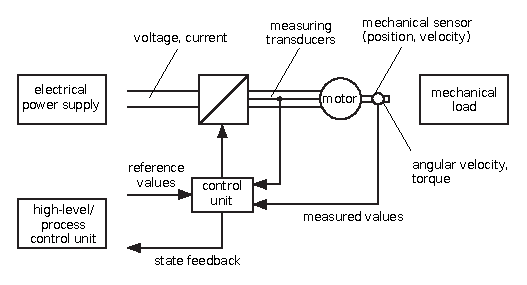
\includegraphics[width=0.8\columnwidth]{sota/electric_drive.eps}
         \caption{Electric drive scheme (See: \cite{Boecker2016})}
         \label{fig:edrive}
\end{figure}

%%Unterschied PMSM von anderen Synchronmaschinen
Among several types of synchronous electric machines \gls{pmsm} devices offer characteristics meeting particularly the demands in industrial and automotive applications.
Their  high efficiency,  high torque/power density and high torque-to-inertia ratio as well as maintenance-free operation make them the optimal choice in most cases.
Like all AC motors the \gls{pmsm} consists of a stator and a rotor.
As it belongs to the group of synchronous motors its rotor cycles synchronously with the frequency of the supply current in the stator.
The distinguishing feature of a \gls{pmsm} contrary to other synchronous machines is the incorporation of permanent magnets embedded in the rotor.
These magnets provide a static magnetic field rotating with the rotor and substitute the supplement by electromagnets.
The advantages are less mass inerta in the rotor due to the lack of windings and less maintenance requirements for the commutator \cite{LeVa2014, Schroeder2007}.

%%Welcher Motor wird verwendet und wie sieht ein Querschnitt aus
The motor considered in this work is a \SI{60}{kW} automotive traction PMSM prototype.
Some of its important components - in particular the stator yoke, stator tooth and permanent magnets - are depicted in fig. \ref{fig:pmsm_cross_section} \cite{WaBo2016}.
\begin{figure}
	\centering
	\def\svgwidth{0.6\columnwidth}
         \import{eps/sota/out/}{pmsm_cross_section.pdf_tex}
         \caption{Cross section of the investigated \gls{pmsm} incorporating interior magnets and concentrated windings (Source: \cite{WaBo2016})}
	\label{fig:pmsm_cross_section}
\end{figure}

%%Gliederung PMSM
Section \ref{ssec:pmsm_basic} introduces the basic modeling and operating constraints \cite{LeVa2014, Schroeder2007} whereas sections \ref{ssec:pmsm_loss_heating} and \ref{ssec:pmsm_thermal_model} give insights to occurring power losses \cite{Kylander1995, Roberts1986, Schroeder2007} and thermal modeling \cite{ BoCa2009, LeVa2014, MeRo1991, WaBo2016}, respectively.

\subsection{Basic Modeling And Operating Constraints}
\label{ssec:pmsm_basic}
%%Spannung und Strom in dq-Koordinaten
Describing the basic behavior of the \gls{pmsm} a coordinate system rotating with the rotor in phase is convenient.
The resulting orthogonal axes are noted $d$ and $q$ where the former is aligned with the rotor's permanent magnetic field.
In steady state, both explain important electric quantities in a time-invariant fashion.
The coordinate system's angular velocity is given by $\omega_{el} = p\omega_{mech}$, where $p$ denotes the pole pair number and $\omega_{mech}$ describes the rotor's mechanical angular velocity.
Neglecting magnetic anisotropy and (cross-)saturation effects the voltage in $dq$-coordinates derives to
\begin{align}
	u_{sd} = R_s i_{sd} + L_s\frac{\dif{i_{sd}}}{\dif t} - \omega_{el} L_s i_{sq} \\
	u_{sq} = R_s i_{sq} + L_s\frac{\dif{i_{sq}}}{\dif t} + \omega_{el} L_si_{sd} + \omega_{el} \Psi_p.
\end{align}
Here, $R_s$ stands for the stator resistance, $i_{sd}$ and $i_{sq}$ for the current on the $d$ and $q$ axis, respectively; $L_s$ denotes the self inductance and $\Psi_p$ represents the permanent magnet flux linkage.
These equations' equivalent circuit diagram is depicted in fig. \ref{fig:eq_pmsm_scheme}.

\begin{figure}
        \centering
        \def\svgwidth{0.7\columnwidth}
        \import{eps/sota/out/}{equivalent_scheme_dq_coordinates.pdf_tex}
        \caption{Equivalent PMSM scheme (See \cite{LeVa2014, Schroeder2007})}
        \label{fig:eq_pmsm_scheme}
\end{figure}
Following this notation, the electromagnetic torque $T$ can be described by
\begin{align}
	T = \frac{3}{2}p\Psi_pi_{sq},
\end{align}
which inherently shows the required $q$-axis current for a desired torque.
As for every physical system, constraints need to be taken into account with one of them being certain limitations for the current and voltage amplitude:
\begin{align}
	|U| = \sqrt{u_d^2 + u_q^2} \leq |U|_{lim}\\
	|I| =  \sqrt{i_d^2 + i_q^2} \leq |I|_{lim}.
\end{align} 
As losses typically scale with the stator current amplitude $|I|$, one would usually opt for minimizing $i_d$ as far as possible, $i_d = 0$ at minimum.
More on losses in the next sections.

Note, that the motor parameters $L_s$, $\Psi_p$ and $R_s$ are not constant over the operation range due to temperature and saturation effects causing the analytical calculations to become unreliable.

\subsection{Power Losses and Heating}
\label{ssec:pmsm_loss_heating}
%%Verlustarten (Welche Verluste treten in PMSM grob auf, weshalb und wo)
Losses in synchronous machines  are divided into two categories based on their source and dependency: Load losses and no-load losses.
As one can infer from their nomenclature, no-load losses are load-independent while load losses strongly depend on the load and the currents.

\subsubsection{No-Load Losses}
%% No-load loss
In particular, the following losses are to be expected at no load:
\begin{itemize}
	\item Iron core losses in the stator teeth and yoke, evoked by the main flux through reversal of magnetism,
	\item losses due to friction and windage and
	\item no-load stray losses and other minor losses.
\end{itemize}
Core losses describe eddy current losses and hysteresis losses, which are proportional to the frequency and the peak flux density.
Calculating these losses is difficult as manufacturing variations, harmonics and temperature affect them significantly.

Losses due to friction typically occur in the bearings and their sealings.
The ratio between the losses in the bearings and those in the bearing sealings are generally not known \textit{a priori}.
Windage losses occur by the incorporation of a cooling fan but as they come with the fan's cooling ability they don't cause an increase in heating.

The last item summarizes those losses of no fundamental frequency e.g. flux harmonics inside the magnets, surface losses or resistive losses due to the no-load current. 

\subsubsection{Load Losses}
%% Load losses
Load losses, on the other hand, consist of resistive losses in the stator winding and losses evoked by the leakage flux and space harmonics.
For a non-sinusoidal supply voltage there are considerable harmonic losses increasing the resistive losses in the stator windings due to harmonic currents and the skin effect.
Furthermore, core and surface losses grow because of the harmonic flux components.

\subsubsection{Heat Transfer}
%% Unterschied conductive and convective
Heat flow is either conductive, convective or based on radiation.
The latter is negligible relative to the former two forms of heat transfer in case of synchronous motors.
Conductive heat transfer happens within solid components and is modeled in a cylindrical rod structure in most cases.
Convection, further, describes transfer processes based on fluid motion (air or liquid).
That could be heat transfer from solid components to the internal air within the enclosed motor and from there, again, to ambient air.
Having a build-in cooling fan or a liquid cooling system, forced convection would boost motor cooling.
Otherwise, convective heat transfer is by free convection only.  

\subsection{Thermal Modeling}
\label{ssec:pmsm_thermal_model}
Naturally, the motor's current-dependent losses and, thus, its heating are primarily influenced by the motor's operation mode.
Typical operation modes are defined in VDE standard 0530 \cite{VDE0530}, which play an important role in the construction of every motor.
However, the thermal environment in automotive applications is challenging and requirements on power density and reliability as well as pricing pressure urge motors to their limits.
High temperatures due to overload will damage the stator windings' insulation varnish and reduce the device lifetime considerably.
Besides that, perseverative high thermal stress degrades the permanent magnets' material and can ultimately lead to their irreversible demagnetization.
Hence, precise thermal analysis became an indispensable tool and thermal management technology experiences growing attention.

The motor is a thermal system consisting of different components in certain constellations (stator, rotor, windings, air gap etc.), where each has its own thermal characteristics.
Analyzing the thermal behavior of this system as a whole is non-trivial.
Nowadays there are two basic approaches to the thermal modeling of electric motors: analytical lumped-circuit (with the optional aid of empirical data) and numerical methods.
Their main differences lay in the required computational time, achieved precision and geometrical limitations.

Regardless of which technique is practiced a designer of thermal models often has to determine thermal resistances beforehand.
Calculating these thermal resistances goes by simple, well established equations for every kind of heat transfer (conduction, convection and radiation).
However, the equations' parameters are partly difficult to define as they depend not only on geometry but also on e.g. fluid turbulence or the interface gap between components.
As a consequence, modeling quality benefits from a designer's experience and the accuracy of material parameter data sheets.

For the numerical approach there are two well established types \cite{BoCa2009}: \gls{cfd} and \gls{fea}.
Regarding the analytical approaches \cite{BoCa2009, MeRo1991, WaBo2016}, the methodology of \glspl{lptn} are described below and their particular shortcomings are worked out in order to motivate this work's purpose.

\subsubsection{Numerical Analysis}
Numerical analyses emerged in the 1990s with the advancements in computational capacities.  
While being capable of modeling any device geometry is a highly appreciated advantage of numerical approaches, the high demand in computational time and model setup prevent them from being of practical use outside the construction phase.
Nevertheless, due to their relatively precise modeling capabilities they play important roles in research and development.

%%FEA
The main purpose of \gls{fea} is the accurate determination of conductive heat transfer within and between solid components of almost arbitrary geometry.
Its time-consuming factors consist of mesh definitions for the model setup and heat-field computations.
Though its application takes a considerable amount of time, it is able to find non-linear loss distributions across the electric machine and a non-symmetrical operational flux density. 
\gls{fea} can also be used as previous step to network analysis for accurate thermal conductivity calculation and to define more accurate loss injections in the network nodes as well as for the determination of the thermal-network discretization level.
There is a thermal and an electromagnetic variant of \gls{fea}, each for its corresponding purpose of analysis, but this does not preclude a combination of both, which can lead to temperature-dependent loss computations.
Unfortunately, similar to \glspl{lptn}, \gls{fea} suffers from imprecise thermal resistance computations and material parameter data.
Moreover, while conductive heat transfer computations are usually excellent, good results are more difficult to achieve for the convective counterpart.

%%CFD
The application of \gls{cfd} principally aims for the computation of the rate and velocity of the coolant flow.
Further it gives evidence about surface heat transfer and pressure distributions in the cooling passages within the machine.
Conversely, \gls{cfd} provides reasonable support for fan design as fans incorporated in electric machines often constitute poor efficiency in an aerodynamic matter due to competitive pressure.
When designing thermal models via \gls{cfd}, building an accurate mesh without excessive cell numbers represents the biggest challenge.
Though it is beyond the scope of \gls{cfd}, there are attempts to model conduction with it, too, yet \gls{fea} is undoubtedly the better choice.
However, the insights gained by \gls{cfd} can help to improve the analytical algorithms in a \gls{fea} model or in thermal networks.

\subsubsection{Thermal Management}
%%Passive thermal management is bad
Although through specification of certain limits to the maximum torque or current rating - including relatively large safety margins - thermal induced damage indeed can be avoided, this will cause an inevitable constraint on the performance.
While rating limits are specified in motor/inverter data sheets they don't take any current temperatures into account and are, thus, mere passive means to thermal management.
Since these limitations have to consider worst-case scenarios, there are several circumstances where large performance potential remains unused. 
When operating at, for example, low ambient temperatures, the heat dissipation capabilities of the components are naturally higher than rated.
In addition, at high operation frequency, junction temperature fluctuations are typically smaller, whereas limiting ratings are defined for the more demanding operation at low frequencies.
Moreover, since fixed current limits account for steady-state operation, the materials' short-time thermal overload capacities can't be utilized. 

%%We need online temperature information
As a consequence, further sophisticated methods should be conducted in order to improve lifetime as well as gaining the maximum performance off the material and utilizing thermal overload capacities without risk of reliability loss.
Here comes online temperature monitoring into play:
online temperature information allows not only safe motor operation but also maximum device utilization in terms of power/torque density.
The naive approach depicts sensor based measurements.
In fact, as pricing pressure is high in the automotive environment and sensors incorporated in particularly rotating parts of an electric machine is tied up with frequent maintenance and error-proneness, this approach is usually not feasible.
Therefore, parametric models with low-computation and less time-consuming properties are the primary choice.
Thermal networks meet those requirements.

\subsubsection{Thermal Networks}
%Thermische Netzwerke (oberflächlich, typische Struktur und Analogien zu el. Ersatzschaltbildern aufzeigen.
Thermal networks show a specific advantage over numerical approaches:
High calculation speeds for low-order networks make the \gls{lptn} suitable for online temperature monitoring.
\glspl{lptn} offer two types of calculation: heat-transfer and flow-network analyses.
The former stands for the thermal counterpart and the latter for the fluid dynamics counterpart to electrical-network analysis.
The equivalences are given in tab. \ref{tab:heat-transfer}.
\begin{table}
		\caption{Equivalences between heat-transfer thermal networks, flow networks and electrical-network circuits}
		\label{tab:heat-transfer}
		\centering
		\begin{tabular}{l l l}
			\toprule
			thermal networks & flow networks & electrical-network circuits \\
			\midrule
			temperature & pressure & voltage\\
			power & volume flow rate & current\\
			thermal resistance & flow resistance & electrical resistance \\
			\bottomrule
		\end{tabular}
\end{table}

In the heat-transfer network thermal resistances would represent main power flow paths between components, which give rise to temperature predictions.
Moreover, thermal networks help defining the necessary discretization level of electric motors.
While in the past relatively simple thermal networks with few nodes were designed, more detailed circuits with more thermal and flow elements can be computed in a fair amount of time today.
A low-order \gls{lptn} is exemplified in fig. \ref{fig:lptn} \cite{WaBo2016}.
\begin{figure}
	\centering
	\def\svgwidth{0.8\columnwidth}
         \import{eps/sota/out/}{lptn.pdf_tex}
         \caption{Example structure of a low-order \gls{lptn} (Source: \cite{WaBo2016})}
	\label{fig:lptn}
\end{figure}

%%Herauskitzeln warum therm. Networks schwierig zu erstellen sind um den Einsatz von NNs besser zu motivieren).
Due to the fact that several thermal phenomena inside electric machines are not analytically solvable in a closed relationship, designing thermal models with sufficient accuracy proves a difficult task even when geometry and material data is known exactly. 
In order to improve prediction performance to an acceptable level, it is common to take empirical data into account to adjust the \gls{lptn} parameters.

Another concern that necessitates experimental measurements is the fact that, in a real-time context, \glspl{lptn} are only feasible in a limited order of complexity.
In other words, the more nodes and elements considered in a \gls{lptn}, the higher the amount of differential equations are subject to computation, which is bounded by the computational capacities of the electronic control unit.
Especially in automotive applications, where the electronic control unit depicts a bottleneck due to its multi-task demands, just relatively small thermal networks prove practical.
Since lower orders of abstraction mean less spatial precision in temperature estimation, those networks rely on additional empirical data in order to not miss hot-spot temperature information.

%%Problem of varying model parameters (e.g. Konvektionswiderstände) bzw. varying model input quantities (e.g. Motor losses and their influencing quantities)
A further problem thermal network designers have to face are varying model parameters e.g. thermal resistances between stator and rotor change due to the motor speed influencing the air gap convection.
Overcoming this problem of linear parameter-varying systems one either has to follow a local approach, where multiple independent experiments are conducted in order to receive a local LTI model for each experiment, or, conversely, one follows a global approach, in which model parameters are directly found through one comprehensive experiment.
For the former, merging all local LTI models together leads to non-robust and possibly inconsistent models, which inherently lack the overload operation range and make the identified \gls{lptn} valid for only a subset of applications.
Going for the global approach, one receives more robust results but this comes with the prerequisite of considering more \textit{a priori} knowledge and predefinition of certain parameter relationships by the model designer.

As developing thermal networks is a demanding task where model designers often have to trade off complexity order (respectively estimation accuracy) against real-time feasibility and where model structures based on heat transfer theory are skewed by the incorporation of experimental data for the benefit of prediction quality, this work investigates the black-box approach of \glspl{ann} as thermal models for electrical traction drives, in particular for the \gls{pmsm}.

%Anwendungskontext (Automobilbereich: Sehr viele exogene Einflussgrößen zB Lastprofil aufgrund Fahrerverhalten, Fahrstrecke bzw. Verkehrslage oder ext. Temperaturen etc). 
%Diese stochastischen Einflüsse erschweren daher das Schätzproblem  und ergeben die Schwierigkeit der Aufgabenstellung.
%Short periods of high demand. Low average power output.

\section{Machine Learning And Artificial Neural Networks}
\label{sec:ml_ann}
%Wo waren sie bereits erfolgreich?
Utilizing \glspl{ann} has proven feasible in many fields of research and often offer state-of-the-art performance.
Especially in the field of automatic speech recognition - both large scale acoustic modeling and language modeling - breakthroughs through the utility of neural networks have called much attention and leveraged their application \cite{GraSchmi2005, SaSe2015, SakHa2014}.
Moreover, there are certain neural network applications in the field of computer vision claiming state of the art in object recognition \cite{LiHu2015}, image generation \cite{GreDa2015} and captioning images/videos \cite{DoHe2014, MaXu2014}.
Furthermore, they have been successfully used in handwriting recognition \cite{DoKo2014, GraLi2009} and in audio analysis \cite{MaFe2014}.
There were even significant advancements in machine translation \cite{LuSu2014} and in predicting protein secondary structure \cite{SoWi2014}. 

A comprehensive and contemporary review of neural networks is given by \cite{Lipton2015}.
The reason for the neural networks' success is attributed to their learning abilities going beyond mere hand-engineered features to learning hierarchical representations and exploiting raw non-determinable features.
The more training and test examples are available for the supervised learning of \glspl{ann} the more does the model benefit from it, as opposed to other models for cognitive and perceptive tasks.
Linear models, for example, tend to under-fit data with a vast amount of data instances and fail to utilize the ever-growing computing capabilities and memory storages nowadays.

%HMMs 
In terms of sequence modeling, \glspl{hmm} represent a considerable competitor to \glspl{ann}.
\glspl{hmm} predict observable sequences given a sequence of unobservable states in a probabilistic fashion.
This is useful in, for example, acoustic modeling, where spoken words are recognized regardless of the speed of speech due to the discreteness of the state space.  
However, HMMs loose their souvereignty quick as soon as the number of hidden states grows large in order to achieve higher expressive power.
Since computing time and the table of transition probabilities rise quadratically with the number of hidden states, computation gets infeasible as of medium-sized state spaces already.
In addition, for the state space being discrete, the expressive capability is even further capped naturally.
Besides that, an important drawback of the \gls{hmm} postulation is the dependency of each hidden state on its previous state only.
This prevents the model to consider long-range dependencies in long sequences, which is essential in plenty of cognitive tasks such as speech recognition, machine translation or any other field where time series have to be predicted.
There have been proposals to extend the accounted context window but they come with a large extra amount of computation condemning the already computation-heavy \glspl{hmm} to perform poorly next to its competitors.

% RNNS too expressive? every NN is differentiable end to end. Gradient based training! There is regularization to prevent overfitting
One important attribute of \glspl{ann}, which differs them from arbitrary models with a similar expressive power, such as a program in C, is the fact that, given the structure and set of its free parameters, they are differentiable end-to-end.
While a written piece of code can theoretically solve any computable task, its search space cannot be explored efficiently.
However, neural networks provide a general way to determine the gradient to the minimization of a chosen loss function with respect to the neural networks' weights, that are its adjustable parameters.
This makes the well studied methodology of gradient-based training applicable.
Furthermore, while present for a lot of models with high expressive capabilities, the problem of over-fitting data during machine learning, that is learning the seen data ``by heart'' without being able to generalize to new data, can be mitigated for the case of \glspl{ann} by several proposed regularization techniques.   

%Wie viel Speicher brauchen NNs auf dem Feld? Wie computational heavy ist deren Einsatz?
Real-time applications benefit from the lightweight utilization of \glspl{ann}.
While training neural networks is computational heavy and time consuming, even more for vast amounts of training examples and bigger nets with a lot of parameters, once training has finished, calculating an output from a given input is significantly faster.

There are diverse architectures leading to varying results in different fields of application and one has to consider each architectures advantages and drawbacks.
The basic \gls{ann}, first proposed in the 1950s, also known as \gls{mlp} or \gls{fnn}, provides undoubtedly the least potential, though it lends itself well for an introduction to the matter.
Aside from the application in the field of computer vision, the \gls{rnn} architecture is the most deployed net among time series modeling tasks together with its variants, for instance, the \gls{lstm}.
Since the \gls{lstm} is frequently applied in this work, it will be explained particularly in the next chapter.
%
%Gliederung
%First of all, in subsection \ref{ssec:basic_topologies} the very basics of \glspl{ann} are introduced and illustrated using the example of a \gls{fnn} and a \gls{rnn}.
%Although not applicable for this work, but nonetheless worth mentionable architectures are outlined as well in subsection \ref{ssec:other_archs}.
%After that, we dive into training neural networks in subsection \ref{ssec:training}, where a brief mathematical derivation is covered.

\subsection{Basic Topologies Of Artificial Neural Networks}
\label{ssec:basic_topologies}
The inspiration for establishing \glspl{ann} was taken from the biological functionality of the human brain.
Each neural network consists of an \textit{input} and \textit{output layer}, one or more \textit{hidden layers}, and a set of \textit{artificial neurons}, also referred to as \textit{units} or \textit{nodes}.
The counterpart to biological synapses are represented by directed edges between the neurons.
Though in the early years of the \gls{ann} history efforts were made to keep the biological analogy, it was soon neglected for the benefit of empirical results.
Each neuron takes arbitrary many input edges and produces exactly one output, which can again be forwarded to arbitrary many other neurons as input.
Moreover, each neuron has a differentiable activation function associated with, which will ensure end-to-end differentiability.
The non-linear function, the neural network is describing eventually, is determined by its set of variable parameters, that are real-valued weights allotted to each directed edge.
It is common practice to allow for an offset weight for each neuron, which further enriches the neuron's expressive power.

Since notation differs throughout the broad range of papers regarding \glspl{ann}, this work sticks to the notation introduced in \cite{Lipton2015} as special emphasis was placed on clean formalities there.
We call a weight associated with an edge from node $j'$ to $j$ as $w_{jj'}$, following a ``to-from'' index notation.
The real-valued output $v_j$ of a node $j$ is the result of its activation function $l_j(\cdot)$ applied to the weighted sum of the node's incoming input edges plus its offset $b_j$:
\begin{align}
	\label{eq:fnn_single_weight}
	v_j = l_j \left( b_j + \sum\nolimits_{j'} w_{jj'} \cdot v_{j'}\right).
\end{align}
Vector notation allows a comfortable description of a whole layer's calculation:
\begin{align}
	\label{eq:fnn}
	\bm{h} = l_h \left( \bm{W}^{hh'} \cdot \bm{h}' + \bm{b}_h \right).
\end{align}
Here, $\bm{h}$ denotes the vector of the current layer's nodes' output values, $\bm{h}'$ those values from the previous layer,  $\bm{W}^{hh'}$ stands for the weight matrix from the previous layer $h'$ to the current layer $h$ and $\bm{b}_h$ notates the current layer's bias vector.
The function $l_h$ represents the activation function for every neuron in the current layer.
Though this is seldom the case, the activation function per neuron can theoretically vary within a layer.
Yet, since this does not apply to most scientific proposals and has no proven benefit, it is assumed here, that each neuron in a certain layer has the same activation function.
The input's and output's data dimension determines the number of neurons in the input and output layer, respectively.

Common activation function candidates are the \textit{tanh} function $\phi(z)=(e^z - e^{-z})/(e^z+e^{-z})$, the \textit{sigmoid} $\sigma(z) = 1/(1 + e^{-z})$ and the \textit{\gls{relu}} $l(z) = max(0, z)$, where the latter was introduced in machine learning research recently with significantly improved results (see \cite{BeBou2013}, for example) giving rise to some other parametric variants.
The activation function of the output layer's nodes is dependent upon the model's purpose.
Having a classification task to solve with $K$ distinct classes, a softmax nonlinearity is applied to $K$ nodes in the output layer, where the output values of all nodes sum to one through the softmax function's normalizing term.
In order to model regression tasks the output nodes' activation function simplifies to the identity function.

Regarding the number of hidden layers: It is mathematically proven, that a standard neural network with just one hidden layer ``is capable of approximating any measurable function to any desired degree of accuracy, in a very specific and satisfying sense.'' \cite{HoSti1989}.
However, it has been shown, that shallow networks often perform insufficiently and plenty of tasks with non-determinable abstract features - especially where the input-output-relation is diffuse - require \textit{deep architectures} with several hidden layers in order to achieve state-of-the-art results \cite{Bengio2009}. Training a deep model is often referred to as \textit{deep learning} and exhibits new challenges in comparison to shallow models.

Within the scope of this work, input and output data always describe temporal sequences.
Hence, further subsections will always point out the impact of specific structures and methods on time series based applications.
Nonetheless, all following observations are also applicable on data without temporal context.

The maximum time index of an investigated data sequence is specified by $T$, yet the case $T \to \infty$ is theoretically not excluded.
Input and target sequences are denoted $\left(\bm{x}^{(1)}, \bm{x}^{(2)}, \ldots, \bm{x}^{(T)}\right)$ and $\left(\bm{y}^{(1)}, \bm{y}^{(2)}, \ldots, \bm{y}^{(T)}\right)$, respectively.
In contrast, a model's predicted output is labeled as $\bm{\hat{y}}^{(t)}$.
Note the superscript in parenthesis to emphasize temporal position as against superscripts without parenthesis for node and layer indices.
Having this terminology set up, an investigated sequence comprises multi-dimensional data points $\bm{x}^{(t)}$ seen by the model one by one in a discrete fashion, where each distinct time step is indexed by $t$.
Each input and target sequence form an example pair and all pairs a full set.
During training the whole considered data is usually called the training (sub-)set. 

\subsubsection{Feedforward Neural Network}
\glspl{fnn}, or \glspl{mlp} synonymously, represent the simplest architecture for neural networks.
They restrict propagation of calculations to one way, from input to output, precluding cycles from higher layers to previous layers or within a hidden layer.
Fig. \ref{fig:fnn} depicts the structure of a simple \gls{fnn} with one hidden layer of three hidden neurons and two neurons for each the input and output layer.
Beginning from the input data $\bm{x}$ each subsequent layer computes its neurons' output values $\bm{h}$, propagates them to the next layer and, ultimately, the output layer returns the result $\bm{\hat{y}}$.
\begin{figure}
	\centering
	\def\svgwidth{0.6\columnwidth}
         \import{eps/sota/out/}{fnn.pdf_tex}
         \caption{\gls{mlp} with one hidden layer}
	\label{fig:fnn}
\end{figure}

The major drawback of \glspl{fnn} is the fact, that they inherently assume consecutive shown data to be independent from each other.
This prevents them from learning any temporal context during learning of sequences or time series.
Yet many important real-world tasks hold temporal dependencies.

\subsubsection{Recurrent Neural Network}
In an attempt to tackle the problem of missing temporal context utilization \glspl{rnn} were introduced.
Their basis is a \gls{fnn} but augmented with timely delayed cycles back to the input of the same layer the cycles have their origin at.
These cycles are called \textit{recurrent} edges and they also include paths from a neurons output to the same neurons input, though they are only attached to hidden layers.
The augmented topology is illustrated in fig. \ref{fig:rnn}, where the neural net holds the same amount of neurons and hidden layers as in the previously exemplified \gls{fnn} structure.
\begin{figure}
	\centering
	\def\svgwidth{0.6\columnwidth}
         \import{eps/sota/out/}{rnn.pdf_tex}
         \caption{\gls{rnn} with one hidden layer (output specifiers omitted to ease clutter). Recurrent edges channel their values at time $t$ back to the layer's input at time $t+1$. }
	\label{fig:rnn}
\end{figure}

Having recurrence incorporated, temporal dependencies find their way to the model.
Analytical calculation is presented for a \gls{rnn} with one hidden layer to keep the matter simple.
At each time step $t$, hidden layer nodes generate an output $\bm{h}^{(t)}$ by receiving current data $\bm{x}^{(t)}$  from the previous layer (here: the input layer) and simultaneously from the same layer's output $\bm{h}^{(t-1)}$ at the earlier time step $t -1$.
The neural network's output $\bm{\hat{y}^{(t)}}$ is thus influenced by the hidden and input layers' nodes' states at previous time steps.
Note, that this topology considers past temporal context only.
Calculating the sole hidden layer's output, equation \ref{eq:fnn} changes to:
\begin{align}
	\bm{h}^{(t)} = l_h\left(\bm{W}^{hx}\bm{x}^{(t)}+\bm{W}^{hh}\bm{h}^{(t-1)}+\bm{b}_h\right),
\end{align}
and for the predicted output $\bm{\hat{y}}^{(t)}$ at time $t$ follows:
\begin{align}
	\bm{\hat{y}}^{(t)} = l_y\left(\bm{W}^{yh}\bm{h}^{(t)}+\bm{b}_y\right).
\end{align}
These equations show temporal indices for the current time step $t$ and the earlier time step $t-1$.
Matrix $\bm{W}^{hx}$ comprises weights associated with the edges from the input layer $x$ to hidden layer $h$, whereas $\bm{W}^{hh}$ and $\bm{W}^{yh}$ explain weights of the recurrent edges and from the hidden layer to the output layer $y$, respectively.
The bias vectors $\bm{b}_h$ and $\bm{b}_y$ represent offset for the respective layers.

In order to support comprehension of the temporal dynamics of a \gls{rnn}, it is possible to unfold the cyclic visualization across time steps.
Fig. \ref{fig:unfold} shows the same simple \gls{rnn} as in fig. \ref{fig:rnn} but with the mentioned principle applied.
This network can be interpreted as deep network with one hidden layer per time step and each layer sharing the same weights.
In this illustration it is highlighted how input data from earlier time steps manages to remain in the network and influences the neural networks' output at a later time step.
\begin{figure}
	\centering
	\def\svgwidth{0.8\columnwidth}
         \import{eps/sota/out/}{unfold.pdf_tex}
         \caption{A \gls{rnn} unfolded across time steps. The highlighted route represents information entering the networks hidden layer, partly remaining there and affecting the networks output at every next time step.}
	\label{fig:unfold}
\end{figure}

\subsection{Other Architectures}
\label{ssec:other_archs}
This subsection shall give an overview of those architectures, which are not investigated in this work.
Emphasis is placed on the motivation and deficiencies of each approach.
The following topologies were not contemplated because either they were not applicable to this thesis' underlying task or would go beyond the scope of this work.
Some of them are simply inferior to other more advanced approaches.

\textit{\glspl{tdnn}} are networks of the feed-forward type, trying to utilize past temporal context \cite{LaWa1990}.
The input sequence is cascaded into successively delayed lines, which act as distinctive features.
Propagating the delayed sequences through the net at once, the topmost layer would receive the whole time window.
Initially introduced to represent a superior approach to \glspl{hmm} in speech recognition, \glspl{tdnn} soon were outshined by its competitor's advancement.

There are certain proposals, where \textit{\glspl{narx}} are combined with \glspl{rnn} \cite{LiBi1996}.
It has been shown, that this particular model may mitigate the vanishing gradient problem of \glspl{rnn} and is capable of learning long-term dependencies two to three times further in the past than mere \glspl{rnn}.
Anyhow, it does not circumvent this fundamental drawback.
Both, \gls{tdnn} and \gls{narx}-\gls{rnn} appear in nowadays scientific papers time and time again, despite their well-known insufficiencies.
One possible reason might be, that these architectures are supported by MATLAB's neural networks toolbox offering an intuitive handling, especially for researchers new to the matter.

An important milestone in neural network research was set with the introduction of bidirectionality to \glspl{rnn}, namely the \textit{\gls{brnn}} and \textit{\gls{blstm}}, which has let to an breakthrough in phoneme classification and handwriting recognition \cite{GraSchmi2005, SchuPa1997}.
Its strength is embodied by the ability to learn context dependencies not just from past data but also from data yet to come during each time step.
Trivially, this comes in handy for applications without real-time demands only, since fixed length sequences are required in the first place.

\textit{Clockwork} \glspl{rnn} \cite{KoGre2014} are a recent alternative augmented by clock rates.
It consists of an \gls{rnn} with one hidden layer, which is partitioned into separate modules, each calculating input data at a different and predefined clock rate.
The purpose of processing sequences at different temporal granularities separately is to address the different dynamic time-scales within time series.

Another novel approach is the \textit{gated feedback} \glspl{rnn} \cite{ChuCa2015}.
It extends the standard topology of deep \glspl{rnn} by global gates between hidden layer pairs, that is, channels from upper layers to the immediately lower layer with adaptive weights.
This further encourages modeling of both, fast changing and slow changing components in the input sequences.
The initiators, \textit{Chung et al.}, want their approach to be understood as a generalization to the clockwork \gls{rnn}, as they embed hierarchically stacked modules across hidden layers, in which the feedback gates adaptively find a proper processing rate.

In the application field of computer vision, \textit{multi-dimensional} \glspl{rnn} were proposed \cite{GraFe2007} performing decent, though they were trumped by \textit{\glspl{cnn}} holding the state of the art until present time \cite{KriSu2012}.
The topology of a \gls{cnn} is of the multi-layered feed-forward category exploiting spatially-local correlation within the input images.
Here, subgroups of neurons are limited to an enclosed, specific receptive field and learn to represent filters or kernels by reacting on certain features at specific spatial positions in the input images. 
One of their strong characteristics is, that they require very little pre-processing of the input images, making their application relatively effortless.

Architectures incorporating an addressable external memory resource are described by e.g. \textit{memory networks} \cite{WesCho2014} and \textit{\glspl{ntm}} \cite{GraWa2014}.
The difference of the former with respect to the latter is a larger memory storage, less complexity and its focus on language and reasoning tasks.
The \gls{ntm} improves upon the capabilities of \glspl{rnn} to solve algorithmic tasks e.g. sorting or copying.
Algorithmic tasks are those, that a simple program could calculate with the very detail of \glspl{ntm} being end-to-end differentiable.
A further advancement is proposed by \textit{pointer networks} \cite{ViFo2015}.
They facilitate attention-mechanics (not outlined in this work, see for example \cite{ChoBa2015, XuBa2015}) as pointer to input elements substituting members of the output sequence.
By doing this, pointer networks are shown to solve sorting tasks with variable sized sequences and certain combinatorial optimization problems.

\subsection{Training Neural Networks}
\label{ssec:training}
The machine learning community separates training into three categories \cite{Bishop2006}:
\begin{itemize}
	\item Unsupervised learning,
	\item Supervised learning and
	\item Reinforcement learning.
\end{itemize}
The first option describes the training of models by giving input training data without corresponding target data.
The expected result is finding coherent subgroups within the data, so called \textit{clusters}, where data members of the same group share more similar attributes rather than those in different clusters.
Other purposes are to estimate the data's probability distribution or to reduce the data's dimension to fewer, more explaining dimensions.
A neural network learning efficient codings during unsupervised learning is called an \textit{autoencoder}.

In contrast, supervised learning represents model learning by ``showing'' corresponding input and optimal target data subsequently, while the model has to find a suitable mapping for it.
If the target data comprises a finite and discrete set of classes, the task is called \textit{classification}.
Conversely, if the target data consists of continuous variables, it is called regression.
Most of the real world applications are of the supervised learning type, which, in addition, is the most investigated machine learning technique for neural networks in terms of published work.

The other category, reinforcement learning, is concerned with finding the best decision given a situation offering several choices against the background of maximizing a reward or, respective, minimizing a penalty.
An example for reinforcement learning is the task of teaching a machine how to play a chess game, where victory corresponds to a reward.

Since this work's underlying task is of the supervised learning type, the other approaches are neglected during the remainder of this thesis.
As mentioned earlier, during learning, the model seeks to minimize the difference between the target $\bm{y}$ and the prediction $\bm{\hat{y}}$, which is dependent on the input data $\bm{x}$ and the current internal parameters (weights).
The distance between target and prediction is measured by a loss or cost function determined by the model designer in beforehand.
Through iterative adjustment of the weights, that is the process of training or learning, the model tries to minimize the penalizing cost.

During a classification task, the cross entropy is the prevailing choice for the cost function.
Nevertheless, there are other losses that prove more constructive in certain applications, e.g. the \textit{connectionist temporal classification} loss for sequence labeling in the field of automatic speech recognition, where alignments between targets and inputs are unknown. 
Solving a regression task, the broad majority of investigations utilizes the \gls{mse}.
Indeed, all common loss functions that are considered in linear regression modeling can also be of use in a neural network application.
The \textit{root mean square error} or the \textit{Huber} loss are alternatives one might think of, which are less sensitive to outliers than the \gls{mse}.

\subsubsection{Error Backpropagation}
There are multiple approaches to exploring the error surface evoked by the difference between target and prediction.
The prevailing method for \glspl{ann} is \textit{error backpropagation} and, particularly for \glspl{rnn}, \gls{bptt}  \cite{ LeBo1998, Lipton2015, Werbos1990}.
By applying the simple chain rule, backpropagation identifies the derivative of the loss function with respect to every weight in the neural network.
Thereupon the weights are tuned accordingly.
Error backpropagation encompasses various optimization techniques confining themselves to calculating the loss' first-order derivative only.
The simplest and moderately common variant is \gls{sgd} in conjunction with combining multiple training examples to mini-batches.
\gls{sgd} is called stochastic, since it does not consider all data for each update step but just one single observation.
The incorporation of mini-batches mitigates the stochasticity.
More on the purpose of mini-batches is addressed in section \ref{sec:opt}.
Neglecting them for now, the \gls{sgd} update equation with the cost function $\mathcal{L}_i$ is described by
\begin{align}\label{eq:sgd}
	\bm{w}\gets\bm{w}-\eta\nabla_{\bm{w}}\mathcal{L}_i 
\end{align}
with $\eta$ being the step size or learning rate and $\nabla_{\bm{w}}\mathcal{L}_i $ the objective's gradient with respect to the weights $\bm{w}$ after having seen the single data pair $(x_i, y_i)$.
The learning rate factor is a crucial parameter, which needs to be defined by the model designer in the first place.
Having a too large learning rate, training would diverge quickly, while a too small rate leads to unnecessarily slow training.

In order to mitigate clutter, the term \textit{net activation} is introduced, representing the sum inside the parenthesis in equation \ref{eq:fnn_single_weight}, that is $a_j =  b_j + \sum\nolimits_{j'} w_{jj'} \cdot v_{j'}$, and shall support following equations.
Before gradients can be calculated, a complete forward pass needs to be conducted, such that we have a value $v_j$ at each neuron and the predictions $\bm{\hat{y}}$ at the output layer.
Then, the distance between target $y_k$ and prediction $\hat{y}_k$ for each output neuron $k$ is determined by the chosen loss function $\mathcal{L}(\hat{y}_k, y_k)$.
Subsequently, by applying the chain rule, the sensitivity $\delta_k$ for output neuron $k$ is defined by
\begin{align}
	\delta_k = \frac{\partial\mathcal{L}(\hat{y}_k, y_k)}{\partial\hat{y}_k}\cdot l'_k(a_k).
\end{align}
Remember, that the activation function $l_k$  for the output neuron $k$ is chosen as identity function, in case of regression tasks.
Beginning with the output neurons' sensitivity, we calculate the sensitivity of each neuron $j$ in the immediately preceding layer by
\begin{align}
	\frac{\partial\mathcal{L}}{\partial a_j} = \delta_j = l_j'(a_j)\sum\nolimits_k\delta_k\cdot w_{kj}.
\end{align}
Applying this calculation for each successive layer yields every node's sensitivity by accounting for the sensitivities of all nodes connected by an outgoing edge from the considered node.
Having produced all values $v_j$ during the forward propagation and all sensitivities $\delta_j$ during the backward propagation, we obtain the cost's derivative with respect to a certain weight $w_{jj'}$ with
\begin{align}
	\frac{\partial\mathcal{L}}{\partial w_{jj'}} = \delta_jv_{j'}.
\end{align}
It becomes evident, that weights with a larger negative impact on the loss function in terms of minimization will experience more fundamental updates than those with less pathological influence.

The principal downside of \gls{sgd} and all its variants is the fact, that it is sensitive to local minima and, thus, the global minimum might never be found.
Furthermore, saddle points cease converging speed as long as step size is set constant.

% vanishing gradient problem
In case of \glspl{rnn}, the optimization is considered as \gls{bptt} because the obtained derivatives also account for the specific time step.
Since the inherent recurrence is also interpretable as infinitely deep topology with shared weights across time steps, a profound problem occurs for the gradient determination.
As the recurrent edge's weight remains the same quantity for every time step, this neuron's input contribution accumulates across time steps.
While the gap between the current time $t$, at which error is calculated, and the earlier time $\tau$, in which the neuron's input provides a contribution to the current time's error, grows large, the corresponding gradients explode or vanish, depending on the recurrent weight being greater or less than one, respectively.
These processes are called \textit{exploding gradient problem} and \textit{vanishing gradient problem}, accordingly.
This prohibits learning long-range temporal dependencies in the training data.
\textit{Pascanu et. al.} deal with this circumstance thoroughly in \cite{PaMi2012}.
A curative solution is given by the incorporation of memory blocks, known as \gls{lstm} (see section \ref{sec:arch}). 

\subsubsection{Methods Incorporating The Cost's Second-Order Derivative}
A presumed advancement to error backpropagation  is the \gls{lm} algorithm \cite{YuWi2011}.
It switches back and forth between error backpropagation and an approximation of the Gauss-Newton algorithm upon the current curvature of the cost surface, which is evaluated through approximated second-order derivatives of the cost function.
When approximating the error function in a quadratic manner is reasonable, the advantageous attributes of the Gauss-Newton method are utilized, which is able to converge directly after the first iteration if a perfect quadratic surface is present.
The \gls{lm} algorithm is more stable than the mere Gauss-Newton algorithm, while converging faster than error backpropagation through the speed up in quadratic environments.
This makes the algorithm very efficient but it also has its drawbacks.
Hessian matrix inversions need to be calculated one or more times per iteration, which is computational heavier and more time consuming the larger the neural network, eventually consuming the whole speed up gained by utilizing the Gauss-Newton algorithm.
Moreover, the Jacobian matrix, which is used for the Hessian matrix approximation, has a size depending not only on the amount of parameters and output units of the neural network but also on the number of features.
This leads the Jacobian matrix storage requirements to let memory cost explode quickly and to counteract the benefit of having more training data.
To make matters worse, the \gls{lm} algorithm is developed for \glspl{mlp} only.
Applying it to \glspl{rnn} is still matter of research.
Nonetheless, the \gls{lm} algorithm is an efficient alternative, as long as the investigated neural network is of limited size and of the feed-forward type.

Another competitor to error backpropagation is \textit{Hessian-free optimization} \cite{Martens2010, SuMa2013}.
Although it leads to competitive results even for deep architectures, it still is an approximation to Newton's method and thus suffers from similar problems as the \gls{lm} algorithm.

